\documentclass[11pt]{article}
\usepackage[margin=1in]{geometry}
\usepackage{amsmath,amssymb}
\usepackage{booktabs,longtable}
\usepackage{graphicx}
\usepackage[hidelinks]{hyperref}
\usepackage{xcolor}
\usepackage{placeins}
\input{numbers.tex}
\IfFileExists{m3_numbers.tex}{\input{m3_numbers.tex}}{}

\newcommand{\real}{Pandora}

\title{XSuM: a generative surrogate of the SBND reconstruction chain\\ trained on the BNB Monte Carlo --- technical note}
\author{L.~Wan\thanks{lwan@fnal.gov}}
\date{\today\ (shipped chain of 2026-11-09; work in progress)}

\begin{document}
\maketitle

\begin{abstract}
XSuM is a per-event surrogate of the SBND simulation and reconstruction chain: given the true neutrino vertex and
the post-FSI final-state particles of an interaction, it samples the record that the cafpyana analysis dataframes
hold for that interaction (whether and how many Pandora slices are truth-matched to it, the slice-level block of
about fifty reconstructed quantities, and the set of particle-flow objects of each slice), in the dataframe format
of the production, so that analyses run unchanged on the surrogated dataframes. The model is trained on the 2026
gen2 BNB + cosmics central-value Monte Carlo (v10\_14\_02\_03) processed with a selection-free cafpyana
configuration written for this purpose. This note describes the chain as shipped, its closure against \real{} on
held-out files, block by block, and then what is wrong: the two open items of a collaborator's CC1p0pi selection,
each traced to its cause. The path to the shipped version is summarised in an appendix.
\end{abstract}

\tableofcontents
\clearpage

\section{Purpose and scope}
\label{sec:scope}

The physics case is forward folding without re-simulation: a cross-section model that was never run through
Geant4, Pandora and cafpyana (another generator, a modified FSI model, a new kinematic region) is transported to
reconstruction level by the surrogate and compared with data or with the nominal MC at that level. The surrogate
does not fix data/MC disagreement; it reproduces the MC detector response, including its flaws, for new inputs.

Scope: XSuM generates the complete reconstruction record, not analysis quantities. Selection flags, BDT scores and
derived kinematics such as $|t|$ are recomputed downstream by the analysers (CC coherent pion: S.~Oh; charged
kaons: T.~Wester; CC1p0pi: M.~Fernandez) from the generated variables. Only generator-level truth is an input: the
true vertex and the post-FSI primaries. No Geant4 quantity (particle end points, lengths, daughters) enters the
models; they are used as a diagnostic reference only (decision 2026-11-07). Generator-internal labels (interaction
mode, CC/NC, $W$, $Q^2$, $E_\nu$, signal flags) are never inputs; they are kept in a label table for holdout
tests. Cosmic-only slices do not depend on the neutrino model and are to be taken from the MC; they are not yet in
the surrogated files. Figure~\ref{fig:io} is the chain as built; Fig.~\ref{fig:gap} is where it stands.

\begin{figure}[p]
\centering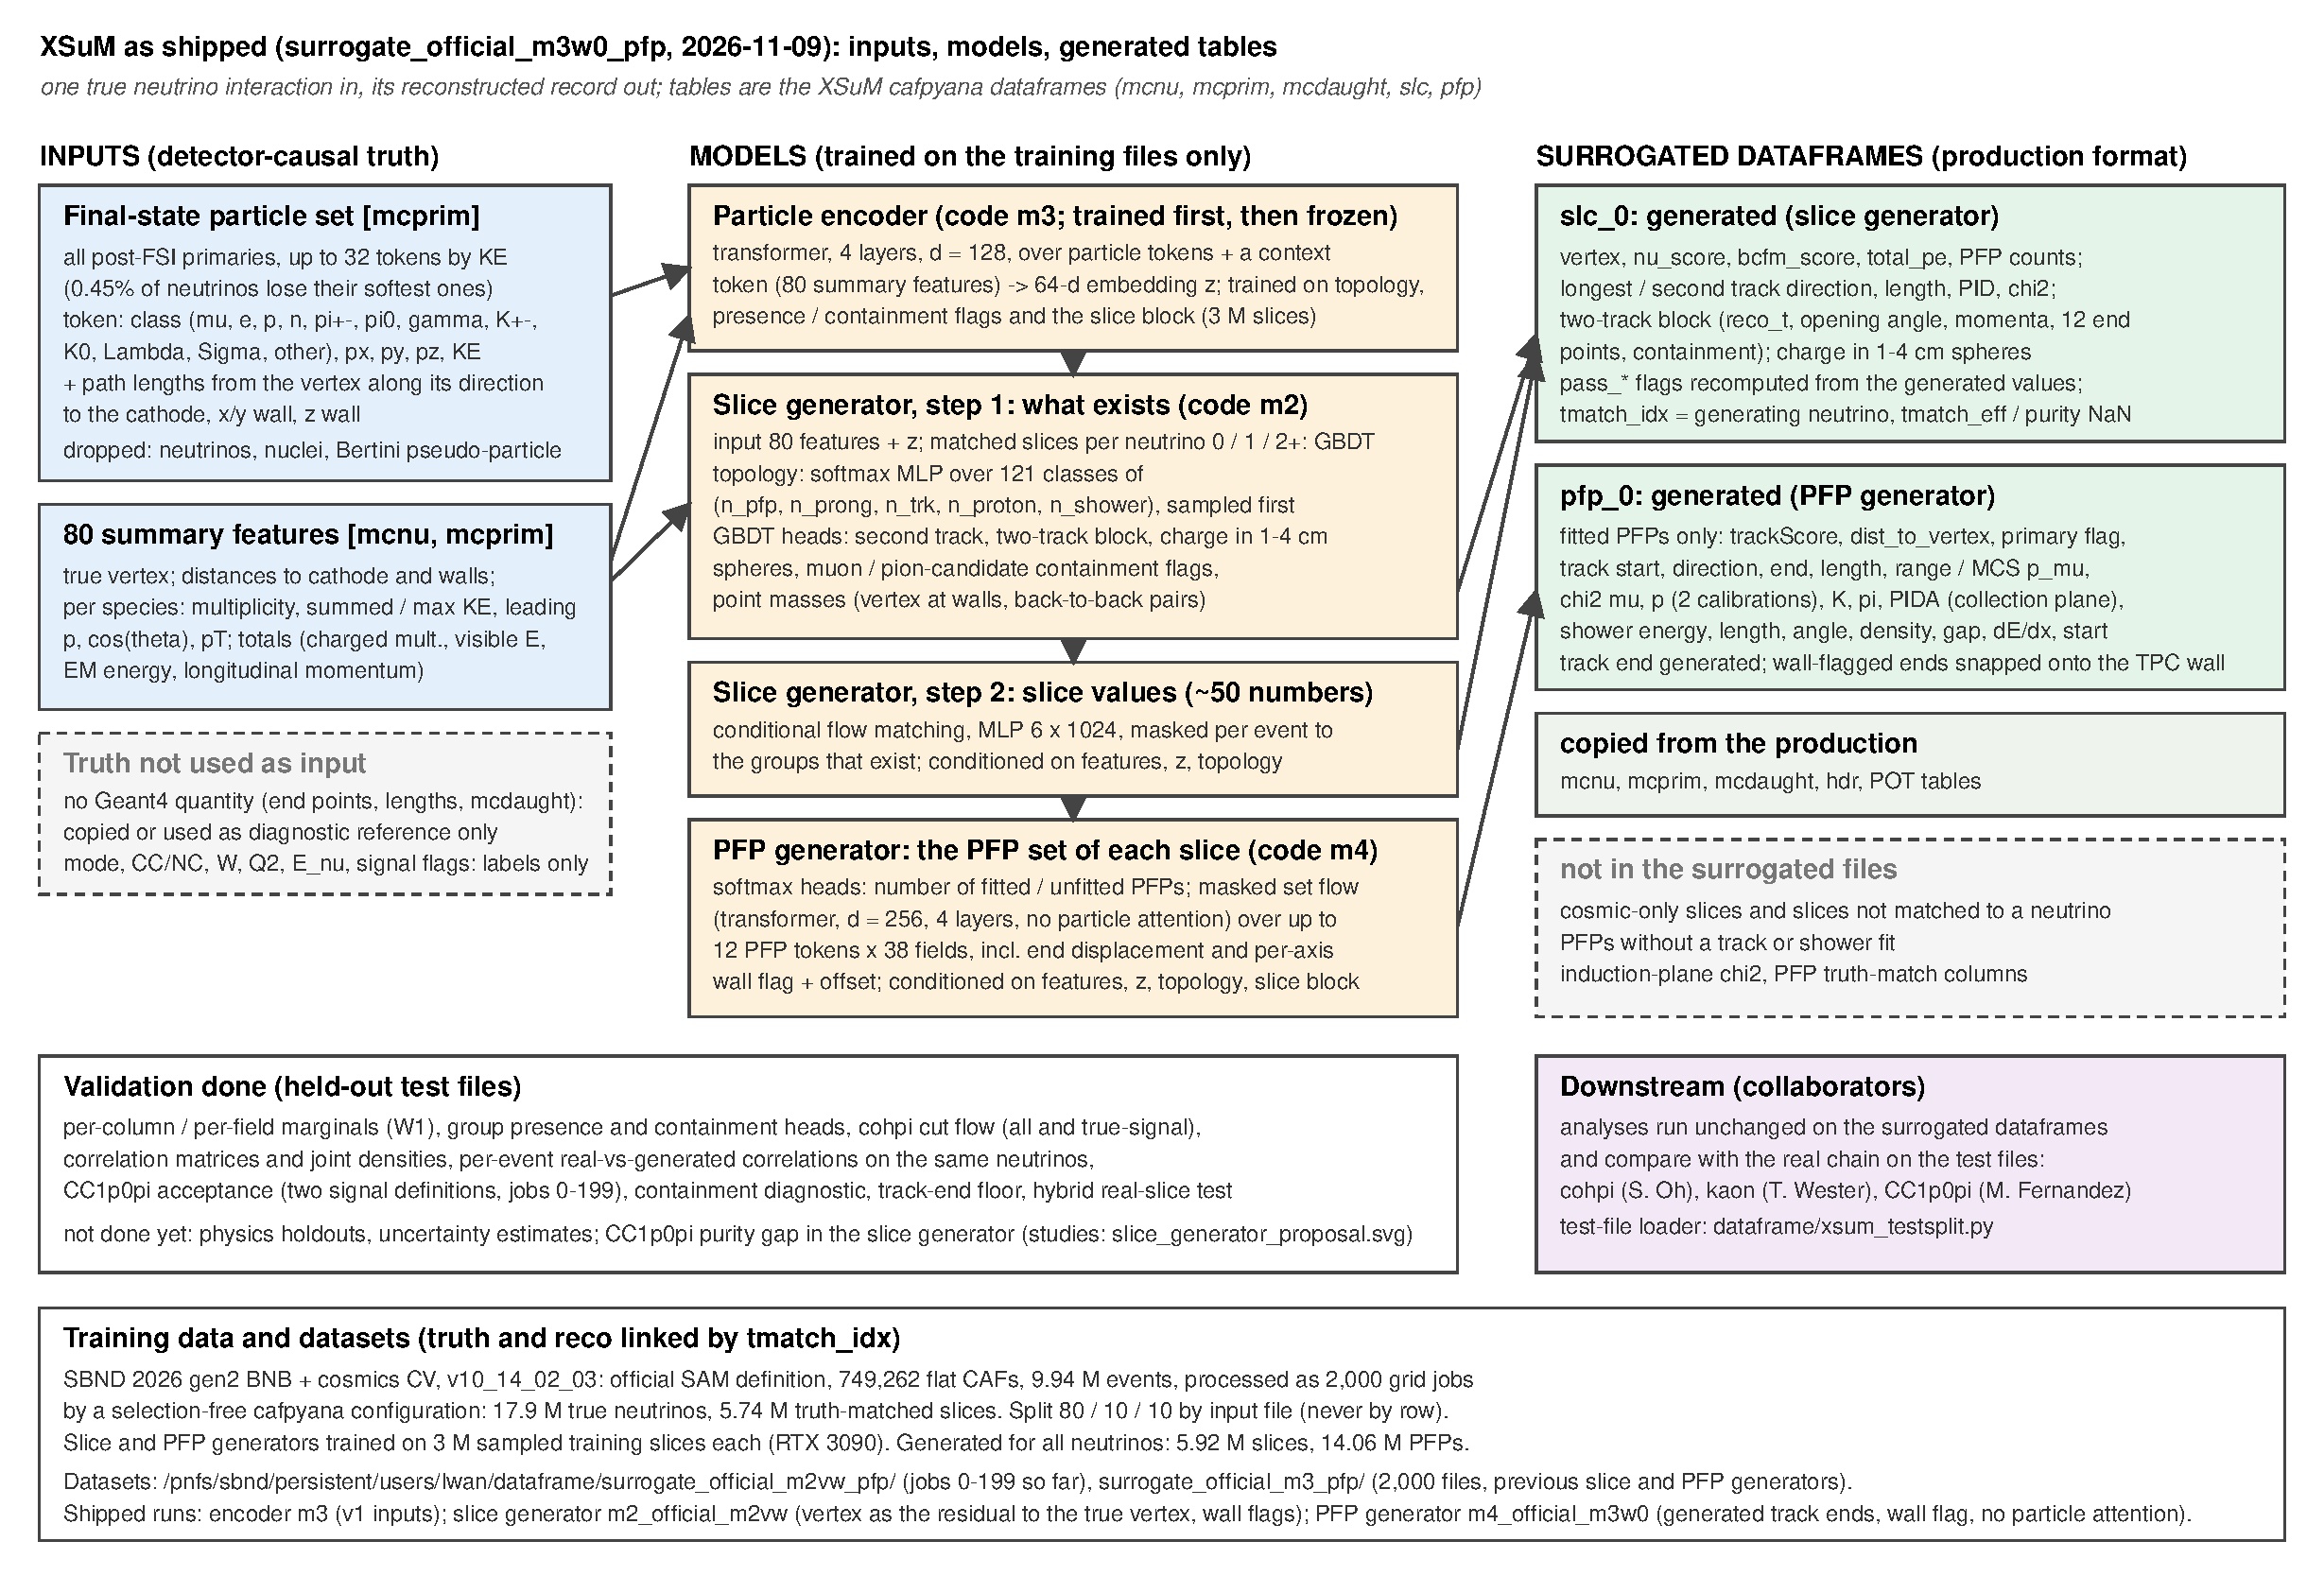
\includegraphics[width=\textwidth]{io_schematic.pdf}
\caption{XSuM as shipped: inputs, the chain of models (particle encoder, slice generator, PFP generator), what the
surrogated files contain (generated, copied, missing), the validation done and the downstream use.}
\label{fig:io}
\end{figure}

\begin{figure}[p]
\centering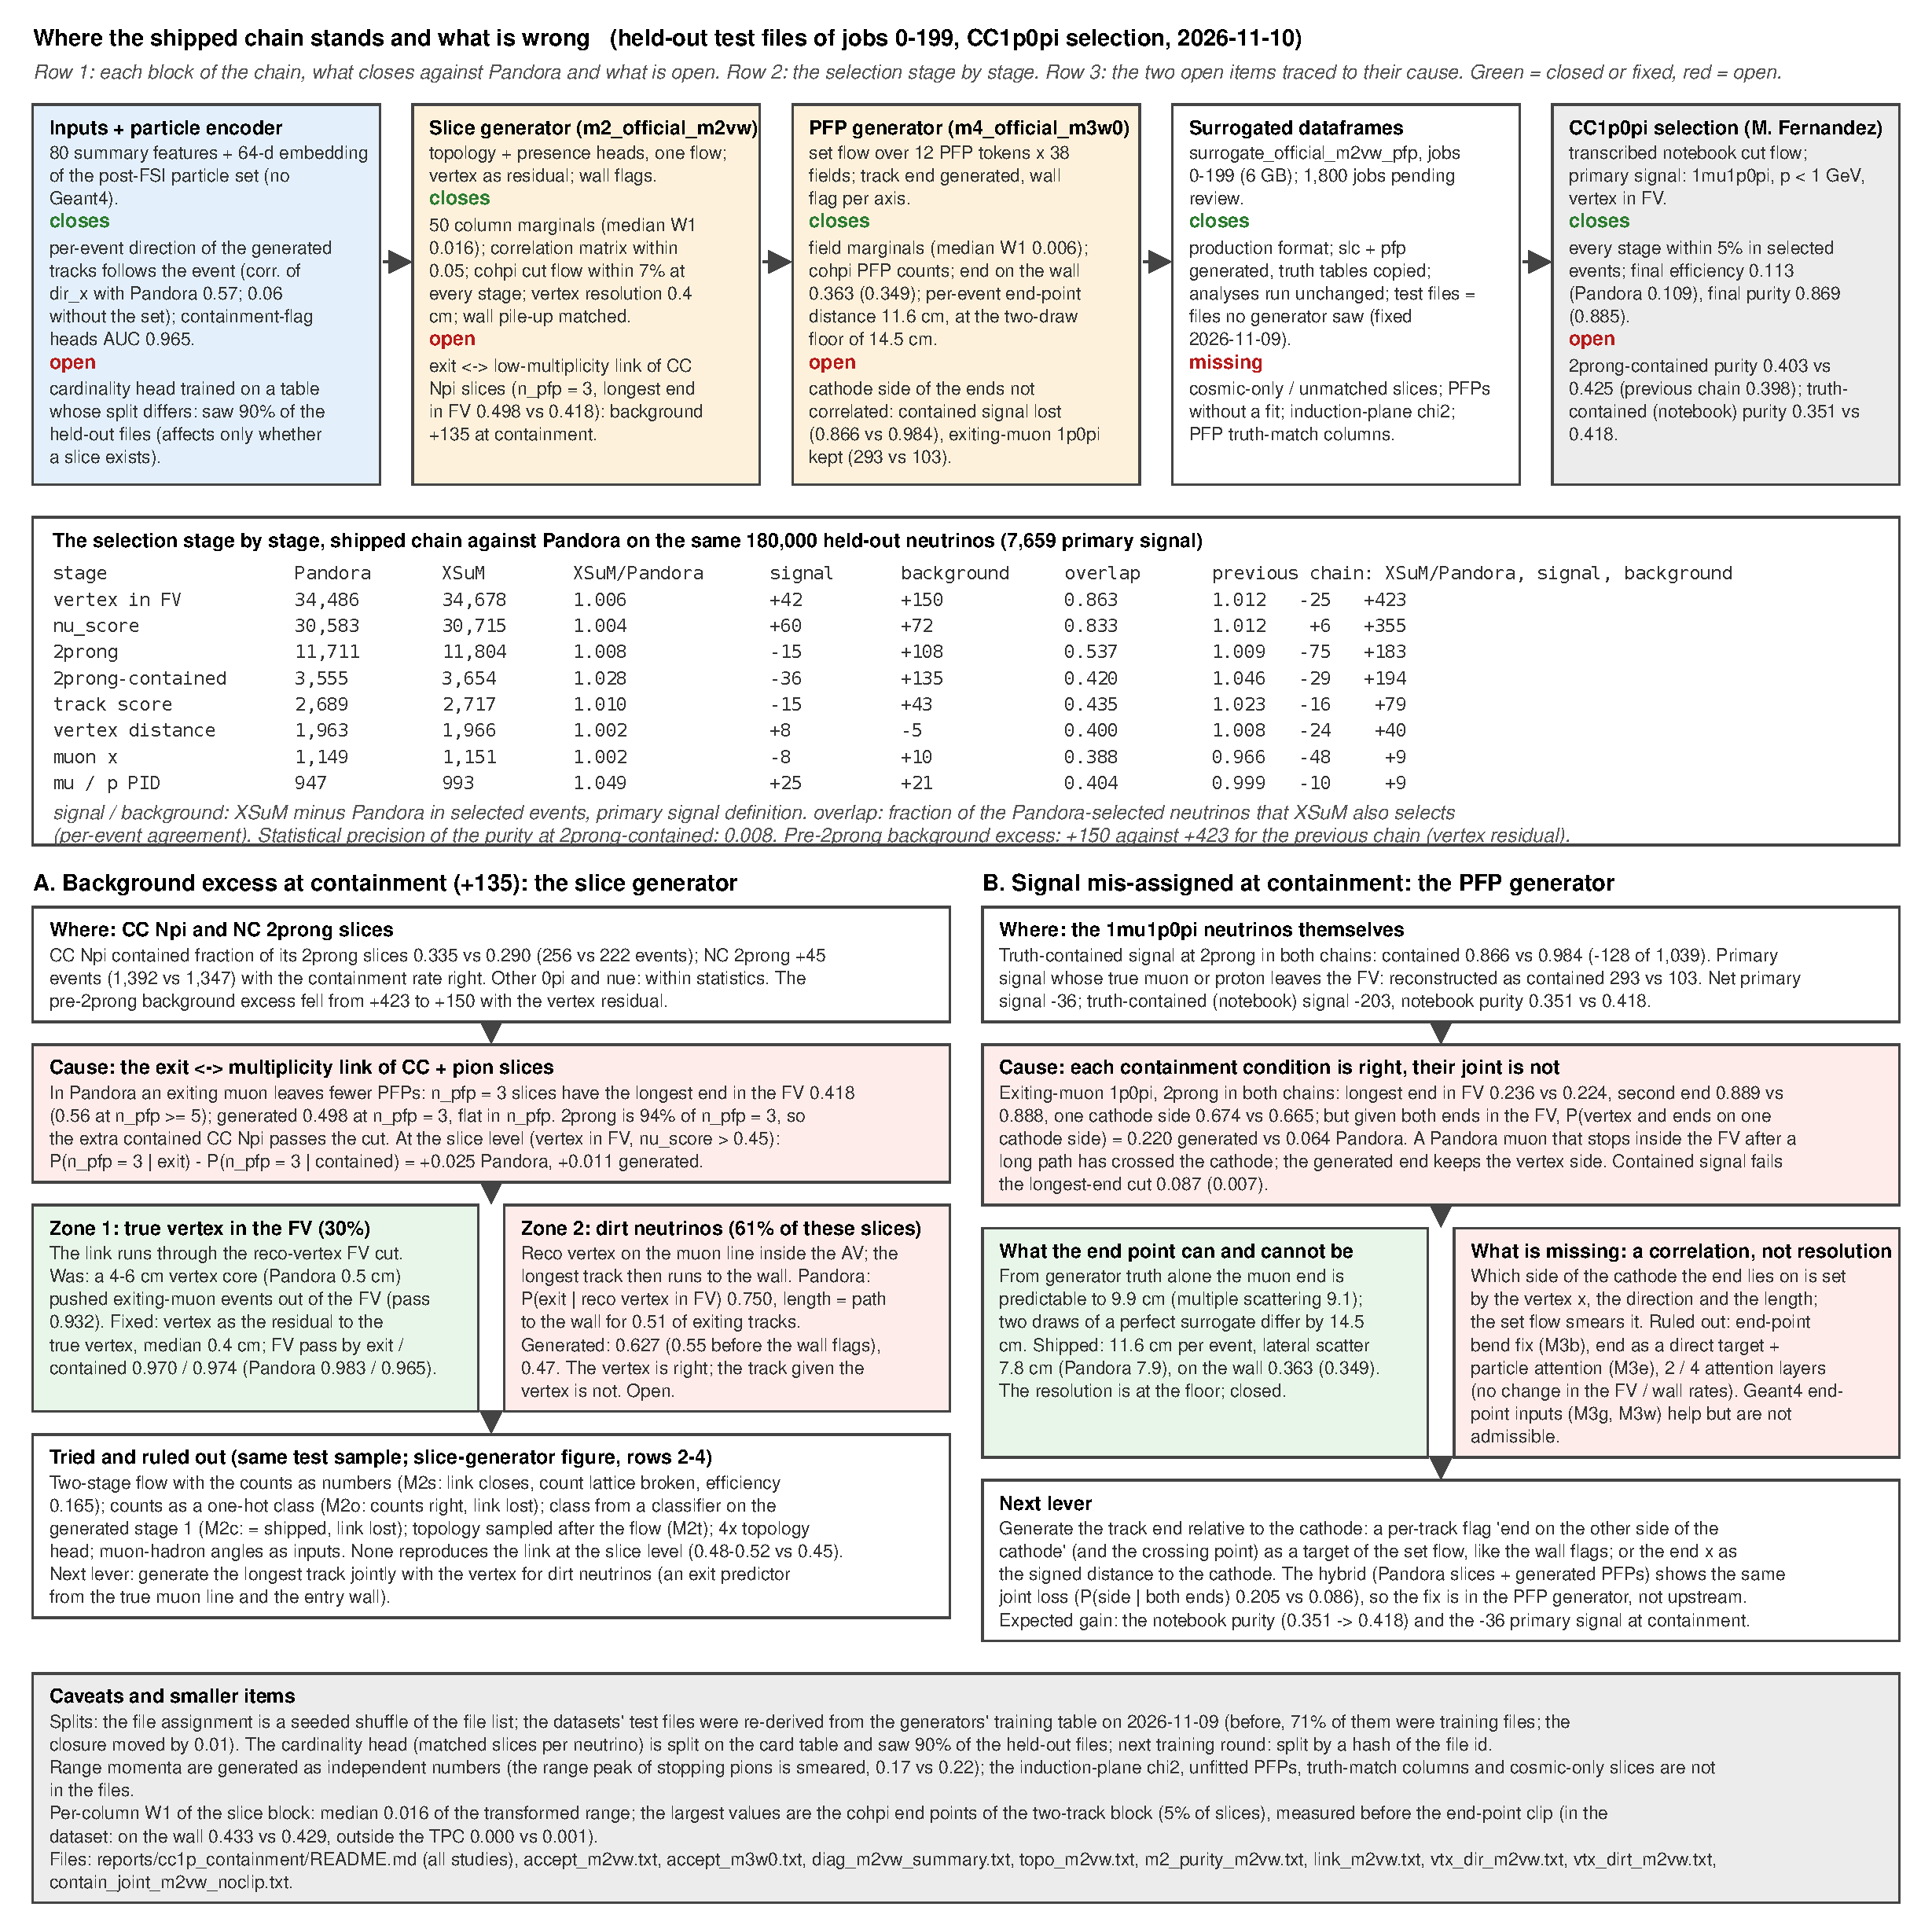
\includegraphics[width=\textwidth]{gap_logic.pdf}
\caption{Where the shipped chain stands on the held-out test files: per block what closes and what is open, the
CC1p0pi selection stage by stage, and the two open items traced to their cause (Sec.~\ref{sec:wrong}).}
\label{fig:gap}
\end{figure}

\section{Data}
\label{sec:data}

\paragraph{Production.} A cafpyana df-maker configuration (\texttt{analysis\_village/xsum/}) writes, per flat
CAF: \texttt{mcnu} (every true neutrino with the full \texttt{make\_mcdf} truth, the cohpi kinematics and
category), \texttt{mcprim} (every post-FSI primary), \texttt{mcdaught} (the Geant4 daughters of every primary),
\texttt{slc} (every non-clear-cosmic slice with the cohpi variables and each selection stage as a flag),
\texttt{pfp} (every PFP of those slices with track, shower and PID variables, kaon PID on all planes, parent
links and truth match), \texttt{hdr} and POT tables. The training sample is the official SAM definition\\
{\scriptsize\path{aurora_SBND2026A_gen2_BNBLight_prodgenie_corsika_proton_rockbox0p1_sbnd_CV_v10_14_02_03_flatcaf_sbnd}}\\
(749,262 flat CAFs, 9.94\,M triggers, 7.9\,TB), processed as 2,000 grid jobs on 2026-10-16 (21.5\,s per file,
4,500 CPU-hours): 17.9\,M true neutrinos (dirt and out-of-volume included), 5.74\,M truth-matched slices. An
earlier scratch production (1,633 merged flat CAFs) served the first models and is retired.

\paragraph{A defect of the official production and its repair.} The module version used on the grid counted
showers among all PFPs of a slice instead of those within 50\,cm of the vertex, so the two-track topology never
fired and the slice two-track block and the selection flags are empty in the archive. All of them are functions
of the PFP table, so they were rebuilt offline exactly as cafpyana computes them (\texttt{xsum.prep.repair}) and
stored as sidecar \texttt{slc} files (the \texttt{slcfix} archive next to the production); the training tables and
the surrogated dataset use the repaired tables, and so must any comparison with the real chain. The module is
fixed for future productions.

\paragraph{Truth--reco link.} A slice points to its truth-matched neutrino through \texttt{tmatch\_idx}; a PFP
points to the true particle it was matched to and, through \texttt{interaction\_id}, to its neutrino. A
neutrino can have zero, one or several matched slices; the table keeps the slice with the highest match
efficiency and records the count.

\paragraph{Splits.} Train / validation / test are 80 / 10 / 10 by input file, never by row. The assignment is a
seeded shuffle of the sorted file list and therefore depends on the whole list: tables with different file lists
get unrelated assignments. The encoder, the slice flow and the PFP generator are trained on the matched table
(745,363 files) and share one split; the datasets' \texttt{file\_splits.parquet} had been derived from the
generated index (13 files fewer) and the cardinality head uses the 4\,M-row card table (740,304 files). Found on
2026-11-09: the datasets' ``test'' files overlapped the generators' test files at 10--20\% only, and 71\% of them
were generator training files. Since then the split table is derived once from the generators' training table
(\path{xsum.data.splits.file_split_table}, \path{scripts/make_file_splits.py}; the 240 files with
neutrinos but no matched slice are test) and copied into every dataset and the test-file loader
(\texttt{dataframe/xsum\_testsplit.py}). All numbers in this note are on that held-out split unless marked
``in-sample'' (the variant comparisons of Sec.~\ref{sec:wrong}, which share the old selection). The held-out
and in-sample closures agree within statistics: the generators do not overfit their training files. The
cardinality head still saw 90\% of the held-out files (it decides only whether a neutrino gets a slice); the next
training round splits every table by a hash of the file id. Holdout tests on physics regions (momentum
transfer, energy, angle, multiplicity, TPC) are listed in Sec.~\ref{sec:next}.

\section{The shipped chain}
\label{sec:chain}

One true neutrino interaction in, its reconstructed record out (Fig.~\ref{fig:io}). Three models, trained in
sequence on the training files of the official sample, one RTX~3090: the particle encoder (code \texttt{m3}, run
\texttt{m3\_official}, frozen), the slice generator (code \texttt{m2}, run \texttt{m2\_official\_m2vw}) and the
PFP generator (code \texttt{m4}, run \texttt{m4\_official\_m3w0}). A writer turns the generated tables into
production-format files.

\subsection{Inputs and the particle encoder}
\label{sec:inputs}

\paragraph{Summary features.} \nFeat{} fixed features derived from the true vertex and the post-FSI primaries
(species, $(p_x,p_y,p_z)$; neutrinos and nuclear remnants dropped): the vertex and its distances to the cathode
and the walls; per species (mu, e, p, n, pi$^\pm$, pi$^0$, gamma, K$^\pm$, K$^0$, Lambda, Sigma) the multiplicity
above the cohpi thresholds (27 / 30 / 20\,MeV for mu / pi / p), the summed and maximum kinetic energy and the
leading particle's momentum, $\cos\theta$ and $p_T$; and totals (charged multiplicity, visible and total kinetic
energy, electromagnetic energy, longitudinal momentum). These features carry no azimuth: with them alone the
generated track directions were uncorrelated with the event (Pearson $+0.06$ in $x$ against \real{} on the same
neutrinos, Table~\ref{tab:m3corr}), so the surrogate reproduced the containment \emph{rate} but not \emph{which}
events are contained, which is what a truth-defined containment signal tests.

\paragraph{Particle set and encoder.} For every neutrino the post-FSI primaries (\texttt{mcprim}; neutrinos,
nuclear fragments and the Bertini binding-energy pseudo-particle dropped) form a set of up to 32 tokens sorted by
kinetic energy (0.45\% of neutrinos have more and lose their softest particles). Each token has a species class
(12 classes) and $(p_x,p_y,p_z,T)$; it is embedded from the class and from its unit direction, $\log|p|$,
$\log T$ and three geometric path lengths from the true vertex along its direction (to the cathode if it heads
towards it, to the nearest $x$/$y$ wall, to the nearest $z$ wall). A context token carries the summary features.
A 4-layer transformer ($d=128$, 4 heads) over the tokens, pooled to a 64-dimensional embedding, is trained on
3\,M matched slices for 6 epochs on the targets that matter for selection: the topology class (cross entropy),
the group presence and containment flags (binary cross entropy) and the continuous slice block (masked mean
squared error); 7\,min. The embedding is frozen and appended to the summary features (144 inputs) for both
generators. Table~\ref{tab:m3heads} shows its effect on the slice heads (the containment flags gain most, muon
candidate AUC 0.892$\to$0.965) and Table~\ref{tab:m3corr} on the per-event agreement of the generated directions
and end points with \real{}.

\begin{table}[h]\centering\small\input{m3_heads.tex}
\caption{Slice-generator heads on the test files with the summary features only (v3) and with the particle-set
embedding added (M3; the shipped generators use it).}\label{tab:m3heads}\end{table}
\begin{table}[h]\centering\small\input{m3_corr.tex}
\caption{Pearson correlation, on the same test slices, between the \real{} value and the generated value, without
(v3) and with (M3) the particle-set embedding.}\label{tab:m3corr}\end{table}
\FloatBarrier

\subsection{The slice generator}
\label{sec:m2}

Generation of the slice record proceeds in three steps. (i) A \emph{topology} head: a softmax classifier over
the joint pattern of PFP counts (\path{n_pfp, n_prong, n_trk, n_proton, n_shower}; the 120 most frequent
tuples plus ``other'', whose members are drawn from the training pool), sampled first; its one-hot encoding
conditions everything that follows. (ii) Gradient-boosted heads for the presence of the variable groups that may
not exist in a slice (second track, two-track block, hits within 1--4\,cm of the vertex), for the two containment
flags, and for the point masses at detector boundaries (vertex pinned at $z=0$ or at the $x$, $y$ walls,
back-to-back track pairs). (iii) A conditional flow-matching model (linear path, Gaussian source, 6-layer velocity
MLP of width 1024) over the standardised continuous block, masked per event to the groups and dimensions that
exist. Positive quantities enter as logarithms, direction cosines and the opening angle through
$\operatorname{artanh}$ (direction vectors are renormalised), standardisation is robust (median, MAD). Two
targets are transformed further. The three reco-vertex coordinates enter the flow as the residual to the true
vertex, $\operatorname{asinh}(\Delta/1\,\mathrm{cm})$, and are added back to the true vertex at generation: as
absolute coordinates under a robust scaling the 0.5\,cm resolution core was hidden next to the 10\,cm-scale
misplacements and came out 4--6\,cm wide. The longest-track length and the cohpi muon and pion end points carry
wall targets, a flag for ``at the wall'' (length equal to the path from the vertex to the wall along the track
direction within 3\%; end point on a TPC wall plane) and an offset within the wall band; at generation flagged
values are snapped onto the wall, the offset clipped to the band, and an unflagged end point beyond the band is
mirrored back inside (\texttt{apply\_walls}, \texttt{tests/test\_walls.py}). A separate gradient-boosted head on
the full neutrino table gives the number of matched slices per neutrino (0, 1 or 2). Inverse transforms produce
a dataframe with the production column names. Trained on \mTwoMatched{} matched slices for \mTwoEpochs{} epochs
(20\,min); host memory is kept near 10\,GB by splitting the table once on disk into a matched-only table and a
4\,M-row subsample for the cardinality head, training the presence heads on 2\,M-row subsamples and building the
topology one-hot per batch on the GPU.

\paragraph{Closure on the test files.} Table~\ref{tab:m2pres} gives the presence and containment heads.
Table~\ref{tab:m2cols} compares every generated column with \real{} (fraction present and Wasserstein-1 in
transformed units; median $W_1$ \mTwoWmed); Fig.~\ref{fig:m2marg} shows the marginals. Table~\ref{tab:m2cut}
recomputes the cohpi cut flow on the generated and the real test slices: all slices agree within 7\% at every
stage; the true-signal column (236 neutrinos) ends at 52 against 67, 1.8 standard deviations. Table~\ref{tab:m2wall}
checks the wall relations of the slice block. Figure~\ref{fig:corrmat} compares the Spearman correlation matrix of
19 slice variables on 250,000 test slices: the generated matrix differs from \real{} by 0.008 on average and by
at most 0.039 (all 167 defined pairs within 0.05; blank cells are pairs undefined because the two-track variables
exist only when \texttt{n\_trk}$=2$). Figure~\ref{fig:corrpairs} shows joint densities of reco--reco pairs,
including the near-deterministic range--length relation, the two-population structure of the vertex charges and
of the proton chi2, and the $|t|$--opening-angle anticorrelation that defines the cohpi signal region.
Figure~\ref{fig:corrtruth} shows the conditional the surrogate exists to learn, reconstructed against true
quantities on the same neutrinos: the exiting-muon band below the diagonal in range momentum, the mirrored band
of muon/pion mis-assignment in the direction, the vertex pile-up at $z=0$ for out-of-volume interactions, and the
two populations of vertex charge.

\begin{table}[h]\centering\input{m2_presence.tex}\caption{Group presence, containment and point-mass heads of the slice generator, test files.}\label{tab:m2pres}\end{table}
\begin{figure}[h]\centering\includegraphics[width=\textwidth]{figures/m2_official_m2vw/m2_marginals.png}
\caption{Marginals of generated against \real{} slice variables, test files.}\label{fig:m2marg}\end{figure}
\begin{table}[h]\centering\input{m2_cutflow.tex}\caption{cohpi cut flow recomputed on real and generated test slices.}\label{tab:m2cut}\end{table}

\begin{table}[h]\centering\small
\begin{tabular}{lcc}\toprule
all matched slices, test files of jobs 0--199 & \real{} & XSuM \\\midrule
longest track: length / path to the wall within $\pm2\%$ & 0.145 & 0.161 \\
\quad length / path $>1.05$ & 0.076 & 0.092 \\
cohpi muon end on the wall ($\pm3$\,cm) & 0.429 & 0.433 \\
cohpi muon end outside the TPC ($<-3$\,cm) & 0.001 & 0.000 \\\bottomrule
\end{tabular}
\caption{Wall relations of the slice block in the shipped dataset (\texttt{scripts/diag\_m2\_purity.py}). Without
the wall targets these read 0.060, 0.133, 0.079 and 0.187.}\label{tab:m2wall}\end{table}

\begin{figure}[p]\centering\includegraphics[width=\textwidth]{figures/m2_official_m2vw/m2_corr_matrix.png}
\caption{Spearman correlation matrices of slice variables, \real{} (left), XSuM (middle), difference (right, scale $\pm0.2$), test slices.}\label{fig:corrmat}\end{figure}
\begin{figure}[p]\centering\includegraphics[height=0.92\textheight]{figures/m2_official_m2vw/m2_corr_pairs.png}
\caption{Joint densities of pairs of reconstructed variables, \real{} (left) and XSuM (right), same test neutrinos, same bins and color scale.}\label{fig:corrpairs}\end{figure}
\begin{figure}[p]\centering\includegraphics[height=0.92\textheight]{figures/m2_official_m2vw/m2_corr_truth.png}
\caption{Reconstructed against true quantities, \real{} (left) and XSuM (right), same test neutrinos.}\label{fig:corrtruth}\end{figure}
\FloatBarrier

\small\input{m2_columns.tex}\normalsize
\noindent The largest $W_1$ values in Table~\ref{tab:m2cols} are the cohpi end points of the two-track block
(present in 5\% of slices); they were measured at training time, before the end-point clip, and the dataset-level
check is Table~\ref{tab:m2wall}.

\paragraph{Generation.} \texttt{scripts/generate\_slc.py} writes slice records for any truth table: slice
cardinality from its head, then topology, presence, point masses and the flow, then the production column names
and the recomputed cohpi flags; about 12,000 neutrinos per second on one GPU, 27\,min for the 17.9\,M neutrinos of
the official sample (5.92\,M slices).
\FloatBarrier

\subsection{The PFP generator}
\label{sec:m4}

The particle-flow objects of a slice are generated as a set. Per matched slice the fitted PFPs (those with a
track or shower fit; the few without either are counted separately) are sorted by distance to the vertex and
padded to 12 (99.99\% of slices have at most 12). Each PFP carries 38 fields: presence flags (track fit, shower
fit, MCS fit, primary), distance to the vertex, track score, start point, direction, range and MCS muon momenta,
chi2 for muon, proton (both calibrations), kaon and pion on the collection plane, PIDA and the chi2 degrees of
freedom, the shower energy, length, opening angle, density, conversion gap and dE/dx, and the track end point:
the displacement end$-$start (3 numbers, generated independently of the direction, so that multiple scattering
can bend the chord away from the initial direction), the excess of the track length over the chord, and per axis
a flag that the end lies on a TPC wall plane with the outward offset from it; flagged ends are snapped onto the
wall at generation. Flags are dequantised, fields that do not exist for a PFP are filled with noise and restored
from the flags after generation. The conditioning vector (\mFourCond{} numbers) is the truth features with the
embedding, the topology one-hot and the generated slice block, so the PFP set is consistent with the slice
record. Two softmax heads give the number of fitted and of empty PFPs; a masked set flow (transformer velocity
net, $d=256$, 4 layers, no PFP-to-particle attention) generates the records. Trained on \mFourN{} slices for
\mFourEpochs{} epochs (45\,min).

\paragraph{Closure on the test files.} The number of fitted PFPs is predicted with \mFourNfitAcc\% accuracy (log
loss \mFourNfitLL{} against \mFourNfitLLm{} marginal): the slice block already carries the multiplicities.
Table~\ref{tab:m4counts} is the physics closure: the cohpi multiplicities (prongs, track candidates, proton
candidates, showers) recomputed from the generated PFPs against the same recomputation on the real PFPs; the
exactly-two-tracks topology rate is \mFourTwoGen\% generated against \mFourTwoReal\% real (\mFourTwoSlc\% from
the slice table itself). Table~\ref{tab:m4fields} compares every generated field with \real{} (median $W_1$
\mFourWmed), Fig.~\ref{fig:m4marg} the marginals.

\paragraph{Track end points.} The end point of the longest track against \real{} on the same neutrinos: 11.6\,cm
per event (3D median; the straight line start $+$ length $\times$ direction 10.0\,cm), lateral deviation from the
straight line 7.8\,cm (\real{} 7.9), end in the FV 0.486 (0.497), on a wall within 3\,cm 0.363 (0.349), outside
the TPC 2.2\% (0.2\%). Signed residuals are below 0.5\,cm on every axis: a resolution, not a bias. How much of it
is intrinsic? Using Geant4 truth only as a reference (\texttt{scripts/diag\_end\_floor.py}), for contained muons
below 1\,GeV the best straight-line prediction from the vertex, direction and range misses the Geant4 end by
9.9\,cm (median; 1.6\,cm from straggling and interactions in the length, 9.1\,cm from multiple scattering in the
direction), and two independent draws of a perfect surrogate differ by 14.5\,cm (median, 90\% quantile 40\,cm).
The shipped per-event distance is at this floor; the target is the distribution, not the event.
PFP-to-particle cross-attention was tested and left out (Table~\ref{tab:attn}): two layers gain 1\,cm and reach
the floor, four add nothing, and the end-in-FV and on-wall rates do not change in any generator-truth class,
while the parameters and the training time double.

\begin{table}[h]\centering\resizebox{\textwidth}{!}{\input{m4_counts.tex}}\caption{cohpi multiplicities recomputed from PFP sets, test slices (counts of slices with 0 / 1 / 2 / 3 / 4).}\label{tab:m4counts}\end{table}
\begin{figure}[h]\centering\includegraphics[width=\textwidth]{figures/m4_official_m3w0/m4_marginals.png}
\caption{PFP fields, generated set against \real{}, test slices (valid tokens).}\label{fig:m4marg}\end{figure}

\begin{table}[h]\centering\small
\begin{tabular}{lcccc}\toprule
particle attention layers & 0 (shipped) & 2 & 4 & \real{} \\\midrule
longest-track end, $|$gen$-$real$|$ median [cm] & 15.3 & 14.3 & 14.2 & 14.5 (floor) \\
\quad straight line start $+$ len$\cdot$dir [cm] & 13.0 & 12.8 & 12.8 & \\
lateral deviation from the straight line [cm] & 9.0 & 8.8 & 8.6 & 7.9 \\
end in the FV & 0.470 & 0.469 & 0.472 & 0.497 \\
end on the wall ($\pm3$\,cm) & 0.355 & 0.363 & 0.359 & 0.349 \\
validation loss & 0.750 & 0.734 & 0.733 & \\
parameters & 2.2\,M & 4.4\,M & 5.5\,M & \\
training time & 7\,min & 20\,min & 25\,min & \\\bottomrule
\end{tabular}
\caption{PFP-to-particle cross-attention ablation (1\,M slices, 15 epochs, no Geant4 inputs), longest track per test slice.}\label{tab:attn}\end{table}
\small\input{m4_fields.tex}\normalsize
\FloatBarrier

\subsection{The surrogated dataframes}
\label{sec:dataset}

\path{scripts/write_surrogate_df.py} turns the generated slices and PFPs into files in the production
format, one \texttt{xsum\_surrogate\_N.df} per grid job $N$ of the archive \path{prod_v10_14_02_03_official/}:
\texttt{mcnu, mcprim, mcdaught, hdr} and the POT tables copied from the production; \texttt{slc\_0} generated
(index \path{(__ntuple, entry, rec.slc..index)}, \texttt{tmatch\_idx} = generating neutrino,
\texttt{tmatch\_eff} / \texttt{tmatch\_purity} NaN, the cohpi \texttt{pass\_*} and \texttt{in\_sr} flags
recomputed from the generated variables, plus \texttt{surrogate\_topology\_class}); \texttt{pfp\_0} generated
(the 38 fields laid out under the production column names, fitted PFPs only, no induction-plane chi2 or
truth-match columns); \texttt{provenance}; and \texttt{file\_splits.parquet}, a copy of the generators' split
(\texttt{--split-table}). Not in the files: cosmic-only and unmatched slices, PFPs without a fit, the
induction-plane chi2 and the PFP truth-match columns.

The shipped dataset is \path{surrogate_official_m2vw_pfp} (2026-11-09), written so far for jobs 0--199
(6\,GB) in \path{/pnfs/sbnd/persistent/users/lwan/dataframe/surrogate_official_m2vw_pfp/}; the other
1,800 jobs follow after review. Next to it, \texttt{surrogate\_official\_m3\_pfp} (2026-11-05, 2,000 jobs,
60\,GB) is the previous slice and PFP generators and remains the only complete dataset until then. Comparisons
with the real chain must use the test files: the loader \texttt{dataframe/xsum\_testsplit.py} reads
\path{dataframe/file_splits.parquet} and the repaired \texttt{slc} sidecars and returns the real and the
surrogated tables of the test files of any list of jobs. Analysers' comparisons so far: cohpi (S.~Oh), kaon
(T.~Wester), CC1p0pi (M.~Fernandez); the last is the acceptance test of Sec.~\ref{sec:where}.

\section{Where we are: the CC1p0pi acceptance}
\label{sec:where}

The collaborator's CC1p0pi cut flow (\path{scripts/check_cc1p0pi_stages.py}, a transcription of their
notebook) is run on the held-out test files of jobs 0--199 of the real production and of the surrogated dataset
(180,000 neutrinos). The stages: a reconstructed vertex in the FV, \texttt{nu\_score} $>0.45$, exactly two prongs
(two good PFP tracks), containment (the vertex and the start and end of both tracks inside the FV and on one side of
the cathode), a track-score cut, a vertex-distance cut, a muon $x$ cut and the muon/proton PID. Two signal
definitions are used. The primary one (decided 2026-11-07): $\nu_\mu$ CC with one muon, one proton and no pions,
$p_\mu$ and $p_p$ below 1\,GeV, true vertex in the FV outside the cathode band, no end-point containment (7,659
signal neutrinos). The notebook's own definition requires in addition the true muon and proton end points inside
one TPC's FV (2,382): that boundary is sharp and set by stochastic end points, so any surrogate with the
end-point floor of Sec.~\ref{sec:m4} moves truth-contained signal out and truth-exiting events in, while the
reconstructed containment cut still selects the same mixture; it is kept as the second table because it is the
analysers' definition.

Table~\ref{tab:accept} gives the result and Fig.~\ref{fig:gap} (second row) every stage with the signal and
background differences. The shipped chain selects within 3\% of \real{} at every stage up to the PID cut (5\%
there), reproduces the final efficiency (0.113 against 0.109) and purity (0.869 against 0.885), and is nearer
\real{} than the previous slice generator at every stage: the background excess before the two-prong cut fell
from $+423$ to $+150$ with the vertex residual. The remaining disagreement is at ``2prong-contained'': purity
0.403 against 0.425 under the primary definition (the previous chain 0.398; the test-sample precision is
$\pm0.008$) and 0.351 against 0.418 under the notebook definition. In events, the surrogate has 36 fewer primary
signal and 135 more background neutrinos at that stage, and 203 fewer truth-contained signal neutrinos.
Section~\ref{sec:wrong} traces the two.

\begin{table}[h]\centering\small\resizebox{\textwidth}{!}{%
\begin{tabular}{lcccc}\toprule
held-out files of jobs 0--199 & selected & primary eff / pur & notebook eff / pur & final stage, primary \\\midrule
\real{} & 3,555 & 0.197 / 0.425 & 0.623 / 0.418 & 0.109 / 0.885 \\
shipped chain & 3,654 & 0.192 / 0.403 & 0.538 / 0.351 & 0.113 / 0.869 \\
previous slice generator, same PFP generator & 3,720 & 0.193 / 0.398 & 0.537 / 0.344 & 0.108 / 0.875 \\\bottomrule
\end{tabular}}
\caption{CC1p0pi at ``2prong-contained'' (selected, efficiency and purity under both signal definitions) and at
the end of the selection (2prong-mup-PID).}\label{tab:accept}\end{table}
\FloatBarrier

\section{What is wrong, and why}
\label{sec:wrong}

Figure~\ref{fig:gap} (third row) is the summary; this section gives the evidence. The diagnostics, all under
\texttt{scripts/}, with their outputs and the full record of the studies in \texttt{reports/cc1p\_containment/}:
\begin{itemize}
\item \texttt{diag\_cc1p\_containment.py}: per neutrino, the two longest good tracks of the \real{} and the
      surrogate slice, each containment condition separately, a generator-truth category;
\item \texttt{diag\_cc1p\_topo.py}: PFP multiplicity against the exit of the longest track, per category;
\item \texttt{diag\_m2\_link.py}, \texttt{diag\_m2\_vtx\_dir.py}, \texttt{diag\_m2\_vtx\_dirt.py}: the slice
      generator on its own test slices, the exit--multiplicity link and the reconstructed vertex by zone;
\item \texttt{diag\_contain\_joint.py}: the containment conditions one by one and jointly.
\end{itemize}

\paragraph{Decomposition.} At ``2prong-contained'' the primary signal is $-36$ and the background $+135$. A hybrid
dataset, \real{} slice table with the generated PFPs (in-sample split), has background $+31$ and signal $-31$ and
recovers the purity (0.426 against 0.435): the background excess comes through the slice block, the signal loss
through the PFP generator. The background excess is in two categories: CC N$\pi$, whose two-prong slices pass
containment 0.335 of the time against 0.290 (256 against 222 events), and NC, with 45 too many two-prong slices
(1,392 against 1,347) at the right containment rate; CC other 0$\pi$ and $\nu_e$ are within statistics.

\subsection{The slice generator: the exit--multiplicity link of CC + pion slices}
\label{sec:link}

In \real{}, a CC N$\pi$ slice whose muon leaves the detector has fewer PFPs: among slices with
$n_\mathrm{pfp}=3$ the longest track ends in the FV 0.418 of the time, against 0.56 at $n_\mathrm{pfp}\ge5$
(\texttt{topo\_m2vw.txt}). The generated slices show 0.498 at $n_\mathrm{pfp}=3$, flat in $n_\mathrm{pfp}$.
Since 94\% of $n_\mathrm{pfp}=3$ slices are two-prong, the extra contained CC N$\pi$ passes the cut. For
1$\mu$1p the two-prong topology is 73\% of the events, so no tail is selected and the same defect does not show.
At the slice level (\texttt{link\_m2vw.txt}, truth CC + pion, reconstructed vertex in the FV,
\texttt{nu\_score}$>0.45$) the link $P(n_\mathrm{pfp}=3\,|\,\mathrm{exit}) - P(n_\mathrm{pfp}=3\,|\,\mathrm{contained})$
is $+0.025$ in \real{} and $+0.011$ generated; without the vertex cut it is absent in both ($+0.005$), so it is
carried by the reconstructed-vertex FV cut. Splitting by where the \emph{true} vertex is
(\texttt{vtx\_dir\_m2vw.txt}) separates two zones.

\paragraph{Zone 1, true vertex in the FV (30\% of these slices), fixed.} The reco vertex passes the FV cut for
0.983 (exiting muon) and 0.965 (contained) of the \real{} slices. With the vertex generated as an absolute
position the generated core was 4--6\,cm against 0.5\,cm and exiting-muon events, whose true vertices lie nearer
the downstream and side walls, were pushed out (pass 0.932). With the residual the displacement median is
0.4 / 0.6\,cm (P($>5$\,cm) 0.175 / 0.307 against \real{} 0.159 / 0.338, tails unchanged) and the pass rates are
0.970 / 0.974.

\paragraph{Zone 2, dirt neutrinos (61\%), open.} For interactions outside the active volume the reconstructed
vertex sits on the true muon line inside the detector (at the entry wall for 0.31, off the line for 0.67) and the
longest track runs from there to the far wall. The position of the reco vertex is reproduced; the track given
the vertex is not (\texttt{vtx\_dirt\_m2vw.txt}): $P(\mathrm{exit}\,|\,\mathrm{reco\ vertex\ in\ FV})$ is 0.750
in \real{} and 0.627 generated (0.552 before the wall targets), and \real{} exiting tracks have a length equal to
the path to the wall within 5\% for 0.51 against 0.47. In the FV-pass table this zone reads 0.296 / 0.112
(\real{}, exit / contained) against 0.248 / 0.166, and it carries $+0.10$ of the $+0.11$ \real{} link.

\paragraph{Tried and ruled out (in-sample split, the same for every row; Fig.~\ref{fig:slicegen},
Table~\ref{tab:variants}).} A two-stage flow with the PFP counts as dequantised numbers in stage 1 (M2s) closes
the link in the chain but breaks the joint count lattice (17\% of slices on tuples \real{} never populates) and
loses two-prong efficiency; with the counts as a one-hot class in stage 1 (M2o) the counts are right and the link
is lost; with the class from a classifier on the generated stage 1 (M2c) the counts and the acceptance equal the
shipped generator and the link is still missing; sampling the topology after the flow (M2t), a $4\times$ topology
head and muon--hadron angles as extra inputs change nothing. None reproduces the link at the slice level (longest
track in the FV for CC + pion $n_\mathrm{pfp}=3$ slices 0.48--0.52 against 0.45). The topology head itself
reproduces the \real{} link when fed the \real{} slice block and loses it on the generated block
(\texttt{diag\_m2\_swap.py}): the link is carried jointly by the longest track, the presence of the optional
groups and the counts, which the generator samples in separate pieces. The next lever is the dirt zone: the
longest track generated jointly with the vertex (an exit predictor from the true muon line and its entry wall),
or the wall relation imposed given the vertex.

\begin{table}[h]\centering\small
\begin{tabular}{llcc}\toprule
run & change to the slice generator & $n_3$ end in FV & eff / pur \\\midrule
\real{} & & 0.439 & 0.198 / 0.435 \\
previous (\texttt{m3}) & summary features $+$ embedding & 0.49 & 0.191 / 0.394 \\
M2w & wall targets & 0.491 & 0.185 / 0.390 \\
M2t & topology sampled after the flow, range on curve & 0.494 & 0.192 / 0.404 \\
M2s & two stages, counts as numbers & 0.442 & 0.165 / 0.396 \\
M2o & two stages, counts as a one-hot class & 0.515 & 0.170 / 0.371 \\
M2c & two stages, class from a classifier & 0.488 & 0.191 / 0.396 \\
M2v & vertex as residual & 0.502 & 0.193 / 0.397 \\
shipped (\texttt{m2vw}) & vertex as residual $+$ wall targets & 0.476 & 0.188 / 0.400 \\\bottomrule
\end{tabular}
\caption{Slice-generator variants, all with the same PFP generator, on the in-sample split: the fraction of CC N$\pi$
$n_\mathrm{pfp}=3$ slices whose longest track ends in the FV ($n_3$ end in FV) and the 2prong-contained efficiency / purity
(test precision $\pm0.008$); the held-out numbers of the shipped generator are in Table~\ref{tab:accept}.}\label{tab:variants}\end{table}

\begin{figure}[p]\centering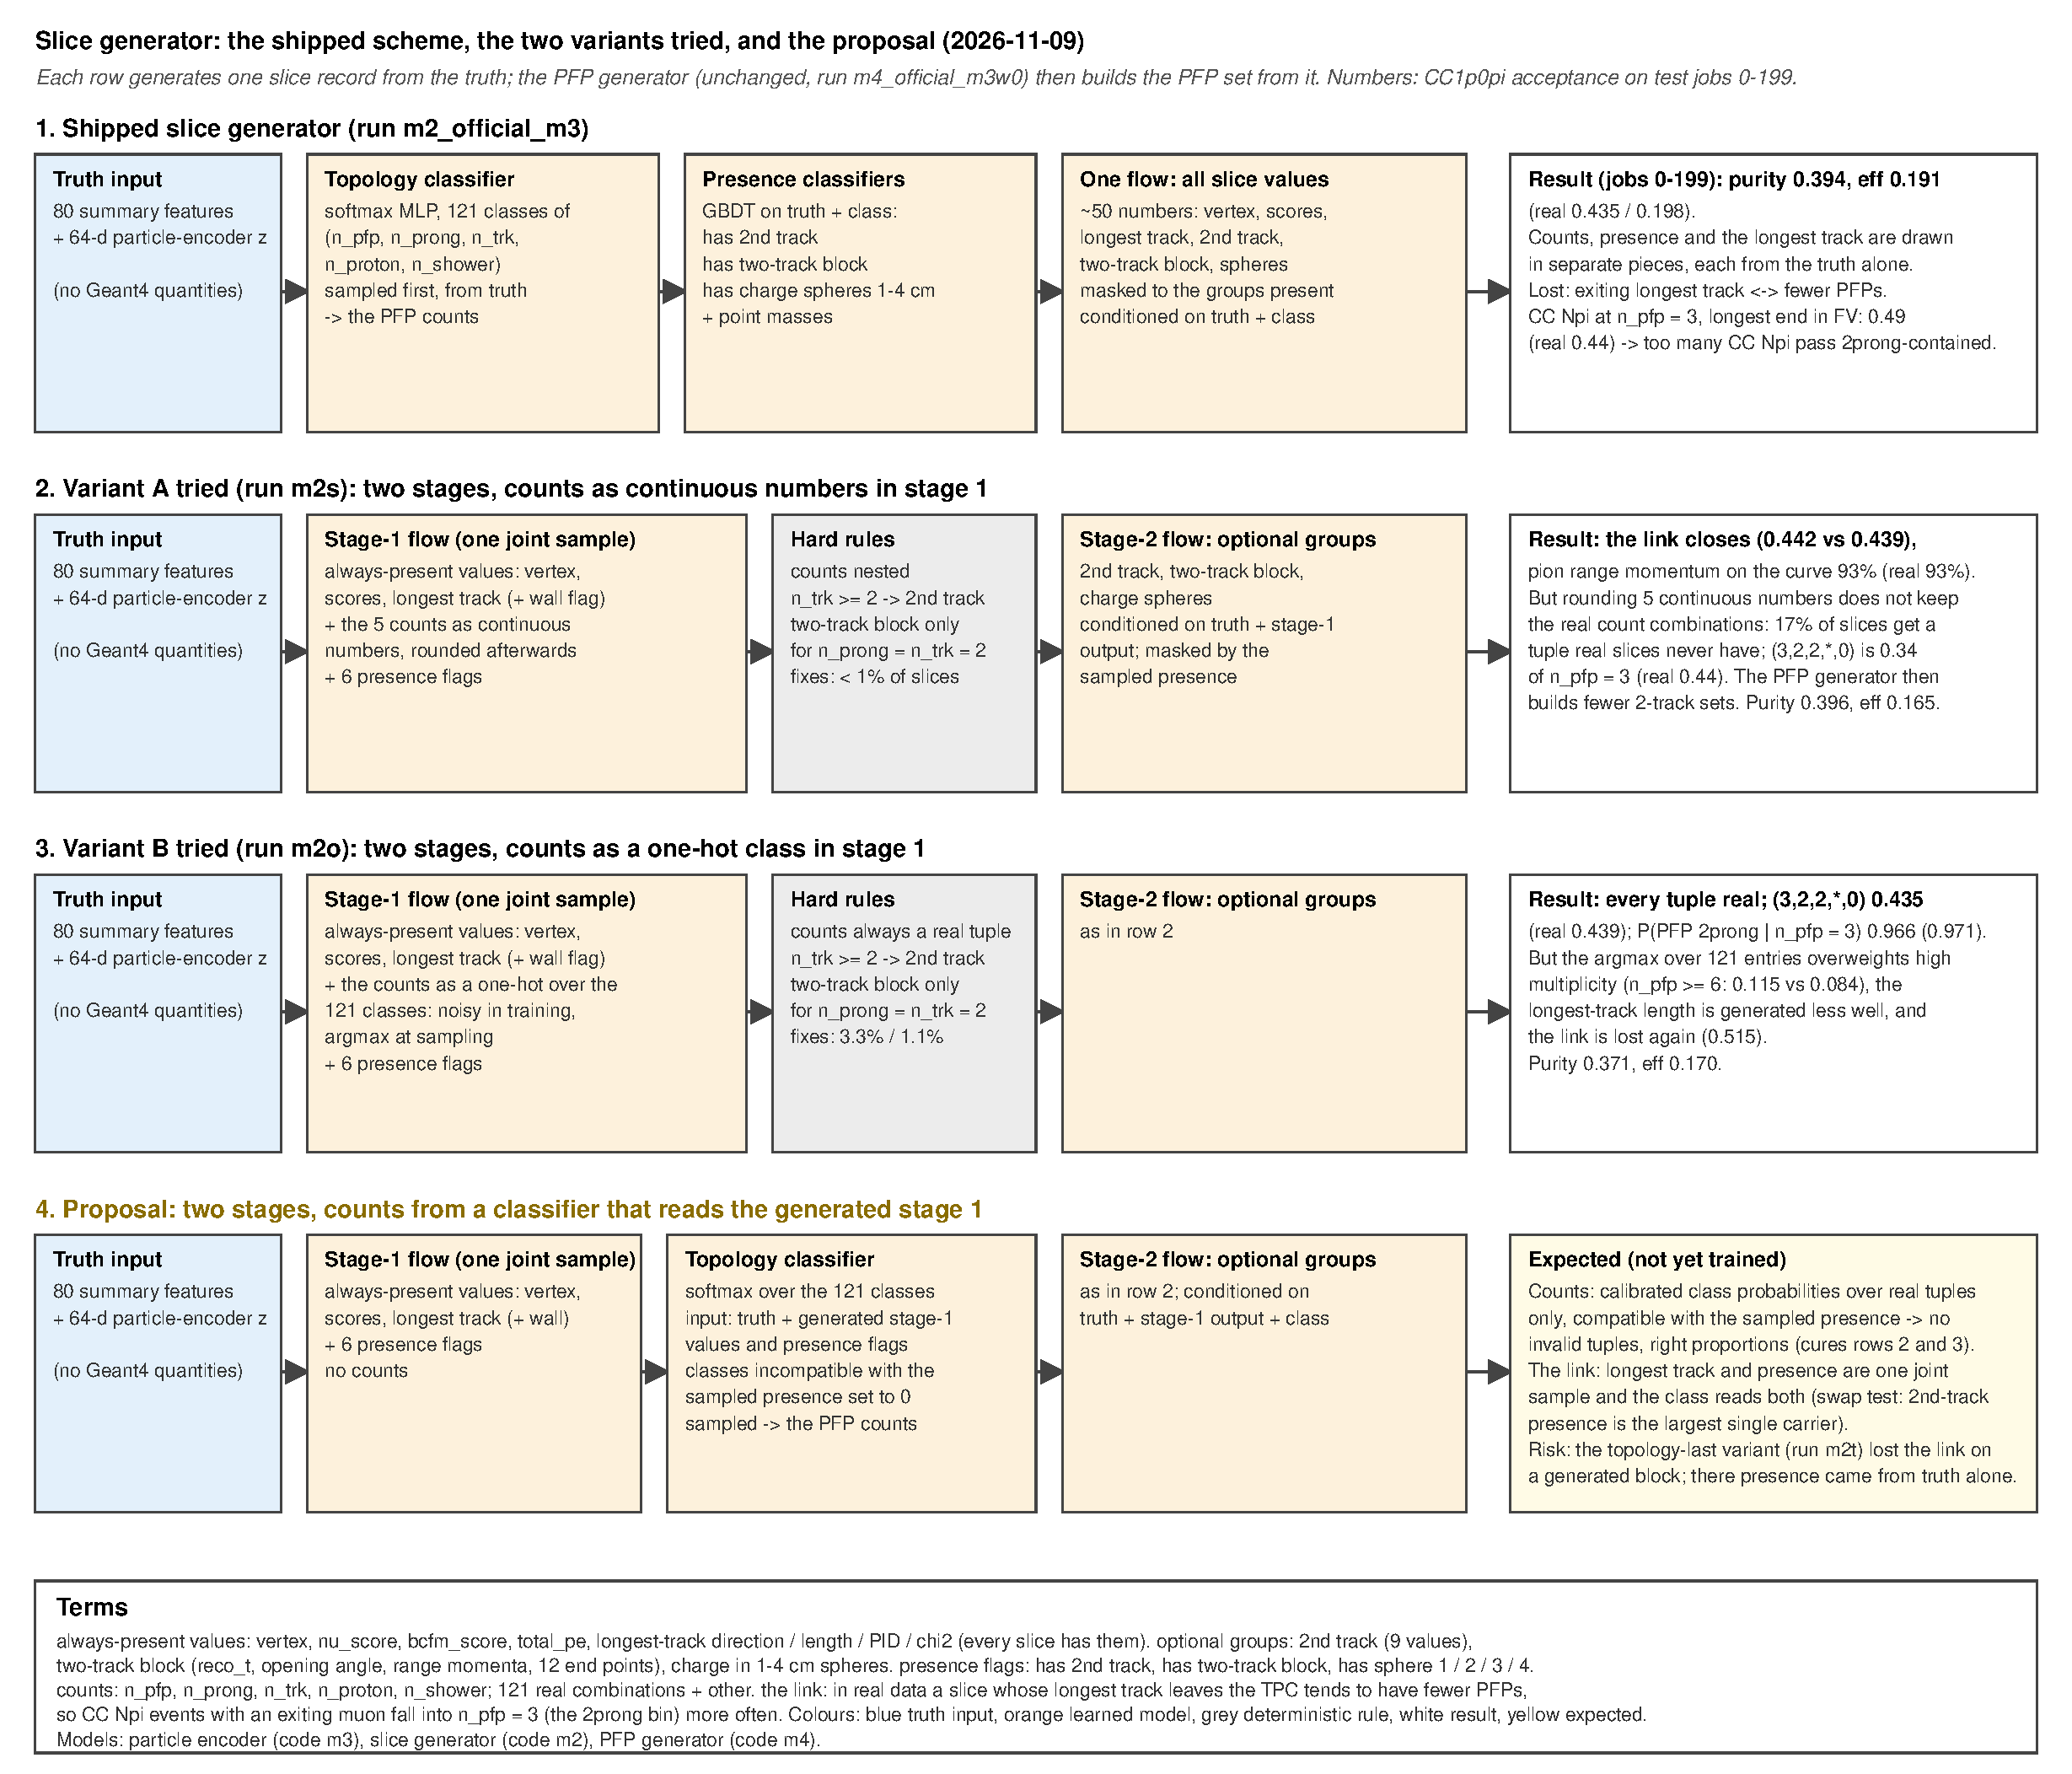
\includegraphics[width=\textwidth]{slice_generator_proposal.pdf}
\caption{The slice generator: the previous shipped scheme, the three two-stage variants, the vertex-residual
variant and the shipped combination, with what each changed (in-sample acceptance numbers).}\label{fig:slicegen}\end{figure}
\FloatBarrier

\subsection{The PFP generator: the cathode side of the track ends}
\label{sec:cathode}

Truth-contained signal neutrinos that both chains call two-prong pass containment 0.866 of the time in the
surrogate against 0.984 in \real{} ($-128$ of 1,039; \texttt{diag\_m2vw\_summary.txt}); the condition that fails
is the longest-track end in the FV (0.087 against 0.007) and, less, the cathode side (0.040 against 0.005). The
mirror image is the primary signal whose true muon or proton leaves the FV: reconstructed as contained 293 times
against 103. Each containment condition passes at the \real{} rate for these events (longest end in FV 0.236
against 0.224, second end 0.889 against 0.888, one cathode side 0.674 against 0.665), but their joint does not:
given both track ends inside the FV, the vertex and the ends lie on one side of the cathode 0.064 of the time in
\real{} and 0.220 generated (\path{contain_joint_m2vw_noclip.txt}). A \real{} muon that stops inside the FV
after a long path has crossed the cathode; the generated end keeps the side of the vertex. The hybrid shows the
same joint loss (0.205 against 0.086), so the defect is in the PFP generator, not upstream. It is a lost
correlation, not resolution: the per-event end-point distance is at the two-draw floor, and the end-point models
tried (a fix of the end-point bend, the end as a direct target with particle attention, two and four attention
layers) left the FV and wall rates unchanged; Geant4 end-point inputs (M3g, M3w) restore the correlation but are
not admissible. The lever is to generate the end relative to the cathode, a per-track flag ``end on the other
side of the cathode'' with the crossing point, as a target of the set flow like the wall flags, or the end $x$
as the signed distance to the cathode. This sets the notebook purity (0.351 against 0.418) and the $-36$ primary
signal at containment.

\subsection{Smaller items}
\label{sec:smaller}

\begin{itemize}
\item The cardinality head is split on the card table and saw 90\% of the held-out files (Sec.~\ref{sec:data}).
\item Range momenta: \texttt{range\_p\_mu} and \texttt{range\_p\_cpi} are functions of the track lengths (97\% /
      93\% of \real{} slices within 2\%), yet the flow generates them as independent numbers and smears the sharp
      range peak of stopping pions (peak fraction 0.17 against 0.22). Flagging them on the curve (M2t) reached 72\%
      on the curve for the pion, the two-stage M2s 93\% (\real{} 93\%); not shipped.
\item Not in the files: cosmic-only and unmatched slices, PFPs without a fit, the induction-plane chi2, the PFP
      truth-match columns.
\item No uncertainty estimate per generated record yet, no physics holdouts yet.
\end{itemize}

\section{Next steps}
\label{sec:next}

\begin{enumerate}
\item PFP generator: the cathode-side target of Sec.~\ref{sec:cathode}; check on the hybrid first.
\item Slice generator: the dirt-zone wall relation of Sec.~\ref{sec:link}.
\item Split every table by a hash of the file id and retrain the chain on it (Sec.~\ref{sec:data}).
\item Write the shipped dataset for all 2,000 jobs once reviewed (pass 2 of \texttt{m2vw\_pfp}); then retire the
      previous complete dataset (\texttt{m3\_pfp}).
\item Range momenta from the generated lengths, with the slice generator's version of the two-track figure.
\item PFP completeness: induction-plane chi2, PFPs without a fit, truth-match columns; cosmic-only and unmatched
      slices from the MC.
\item Uncertainty: Bayesian last layers or ensembles, an out-of-support flag per generated record.
\item Holdouts: train on $|t|<0.1$, test the tail; low versus high $E_\nu$; forward versus wide-angle muons;
      $\le2$ versus $\ge3$ charged primaries; one TPC versus the other.
\item Collaborators' comparisons (cohpi, kaon, CC1p0pi) on the test files of \path{surrogate_official_m2vw_pfp}.
\end{enumerate}

\appendix
\section{The path to the shipped version}
\label{sec:history}

Kept for traceability; the numbers are those recorded at the time (in-sample split before 2026-11-09).
\begin{description}
\item[Baselines (M1).] Gradient-boosted classifiers and mixture density networks on the 80 summary features set
      the floor for every target: slice efficiency AUC 0.977 (32\% of all true neutrinos have a matched slice),
      PFP multiplicity accuracy 56\% against 32\% marginal, and conditional marginals of the vertex, leading-track
      and two-track variables. The code remains (\texttt{xsum.train.baselines}).
\item[Slice generator v1--v3.] v1 (unbounded cosines, counts as dequantised flow dimensions) closed the cohpi cut
      flow only to 45\% in the signal region; v2 (bounded cosines, point-mass heads) to 74\%, losing most at the
      exact-count stage; v3 (topology head, 2026-10-22) to better than 10\% at every stage. v3 with the
      particle-set embedding (\texttt{m2\_official\_m3}, 2026-11-05) fixed the per-event directions
      (Table~\ref{tab:m3corr}; CC1p0pi two-prong-contained efficiency 0.387$\to$0.543 under the notebook
      definition); the vertex residual and the wall targets (\texttt{m2\_official\_m2vw}, 2026-11-09) completed
      it (Sec.~\ref{sec:link}).
\item[PFP generator v2 to M3w0.] v2 (29 fields, end as start $+$ length $\times$ direction) shipped with
      \texttt{surrogate\_official\_v3\_pfp}; the particle-set inputs (M3) and then the generated end point with the
      per-axis wall flag and offset (layout v4, M3w0, 2026-11-08) followed. Models tried on the end point: M3b (a
      fix of the end-point bend) and M3e (the end as a direct target plus cross-attention) left it unchanged;
      M3g (Geant4 start, end, length and containment on the particle tokens; error 20$\to$7\,cm) and M3w (Geant4
      straight-line exit point and wall flag) are not admissible and were kept as diagnostics only. The in-sample
      acceptance at two-prong-contained: M3 0.199 / 0.397, M3w 0.190 / 0.395, M3w0 0.191 / 0.394, hybrid
      (\real{} slices $+$ M3w0 PFPs) 0.194 / 0.426, \real{} 0.198 / 0.435.
\item[Datasets.] \texttt{surrogate\_v3\_6ch} (scratch production, slices only), \texttt{surrogate\_official\_v3}
      (2026-10-22, slices only, 2,000 jobs), \texttt{surrogate\_official\_v3\_pfp} (first dataset with every
      reconstructed object surrogated) and \path{surrogate_official_m3w0_pfp} (jobs 0--199) are deleted
      (2026-11-09); \texttt{surrogate\_official\_m3\_pfp} remains until the shipped dataset is complete.
\item[Signal definition.] The notebook's truth-contained signal was replaced as the primary definition on
      2026-11-07 (Sec.~\ref{sec:where}); the test-split finding and fix are dated 2026-11-09 (Sec.~\ref{sec:data}).
\end{description}

\end{document}
